\section{Evaluation Practices and Evidence Maturity}

The reviewed sources include conceptual architectures, analytical models, simulations, prototypes, datasets, and domain demonstrations. Each form answers a distinct question: security analysis exposes protocol assumptions; network simulation explores scale; blockchain prototypes measure implementation behavior; and field trials examine integration under specified operating conditions. The framework below organizes these forms for future evaluation of mission-trust claims. It does not estimate their prevalence across the literature or report an integrated evaluation of OAL.

\subsection{A Claim-Specific Evidence Profile}

Figure~\ref{fig:maturity} proposes six complementary evidence categories spanning conceptual work, analysis, and operational experience. The numbering is an organizing convention, not a cumulative quality score: formal analysis, experimental control, environmental representativeness, and operational duration are distinct dimensions. A field trial need not contain a formal proof, and deployment does not establish resistance to an untested adversary. Each claim therefore receives an evidence profile identifying the methods used, system scope, assumptions, and conditions tested; one highest category cannot summarize an entire system.

\begin{figure}[!htbp]
\centering
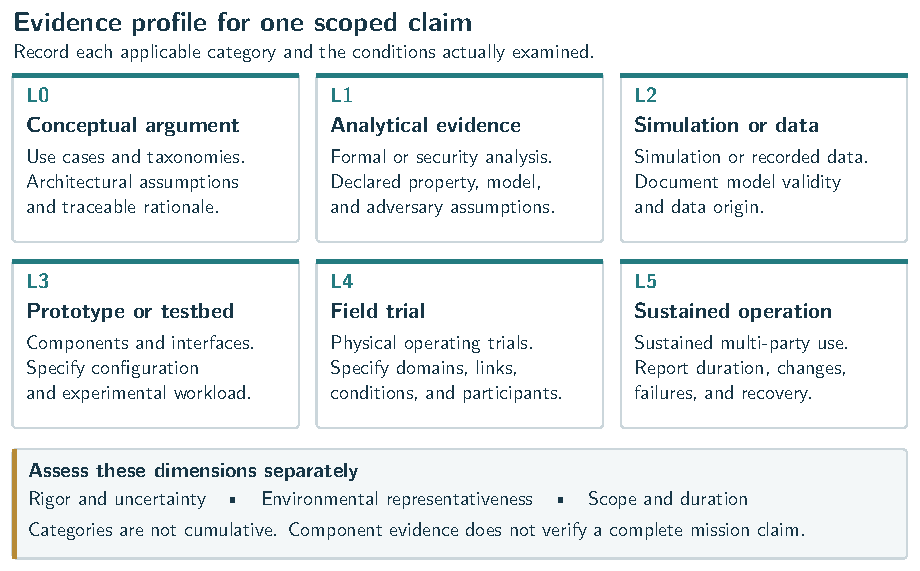
\includegraphics[width=\textwidth]{figures/figure-07-evidence-maturity.pdf}
\caption{Authors' claim-specific evidence profile. The six categories indicate the setting and method supporting a claim; they do not imply cumulative verification or a ranking of scientific rigor.\label{fig:maturity}}
\end{figure}

Category L0 denotes a use case, taxonomy, or architecture supported by conceptual argument. L1 denotes mathematical, formal, or security analysis with explicit adversary and system assumptions. L2 denotes simulation or recorded-data analysis; the origin and representativeness of the data are recorded separately. L3 denotes an implementation tested in a prototype or testbed with a documented configuration and workload. L4 denotes trials under specified physical operating conditions, identifying which vehicle domains, communications, and participants were represented. L5 denotes sustained multi-party operation, with duration and observed governance changes, credential rotation, failures, audits, and recovery reported explicitly. A ledger-throughput test supplies prototype evidence for that component; it does not establish observation validity or mission safety. Integrated claims require evidence for each consequence-relevant dependency, including the interfaces between components.

\subsection{Datasets, Simulators, and Testbeds}

Existing public resources provide candidate components for a cross-domain evaluation environment. TON\_IoT combines labeled IoT/IIoT telemetry, operating-system logs, and network traffic collected in the UNSW Canberra cyber range; Edge-IIoTset uses a purpose-built seven-layer testbed and supplies baselines for centralized and federated learning \citep{alsaedi2020ton,ferrag2022edge}. Together with CICIoT2023 \citep{neto2023ciciot2023}, they support device/link anomaly experiments. Transferring these experiments requires a separate model of maritime topology, physical degradation, and mission consequence. SeaDronesSee provides maritime UAV imagery and metadata for visual detection and tracking experiments \citep{varga2022seadronessee}; evaluating observation validity additionally requires defined physical claims and appropriate ground truth. The supervised GNSS study of \citet{semanjski2020use} trains on synthetically manipulated signals and validates on two distinct real-world spoofing/meaconing datasets, contributing evidence for the evaluated signal features and recording contexts.

The original AirSim study describes a high-frequency physics engine, visual environments, and real-time hardware-in-the-loop support, with selected software components compared against real flights \citep{shah2018airsim}. UUV Simulator extends Gazebo/ROS with hydrodynamics, thrusters, sensors, external disturbances, and multi-robot scenarios \citep{manhaes2016uuv}, while Aqua-Sim NG ports underwater-network functionality to ns-3 and evaluates the redesigned simulator architecture \citep{martin2017aqua}. These resources address complementary components: air-domain perception and dynamics, underwater robot simulation, and underwater communication protocols. Coupling them is proposed integration work, requiring compatible software versions, time synchronization, shared geometry, validated channel interfaces, and reproducible event exchange. Attestation, provenance, consortium behavior, and mission-loss modules must also be implemented and validated; combining the tools alone supplies no ground truth for those claims.

\begin{table}[!htbp]
\caption{Evaluation resources and transfer limits. OAL uses and metrics are proposed evaluation requirements, not results established by each resource.\label{tab:evaluation}}
\begin{adjustwidth}{-\extralength}{0cm}
\scriptsize
\begin{tabularx}{\fulllength}{@{}P{33mm}P{34mm}P{40mm}YY@{}}
\toprule
\textbf{Resource/practice} & \textbf{Primary evidence} & \textbf{OAL use} & \textbf{Important metrics} & \textbf{Required complement}\\
\midrule
CICIoT2023, TON\_IoT, Edge-IIoTset & Labeled network, host, sensor, and attack telemetry; centralized/federated baselines & Device/link anomaly and uncertainty methods & Detection by class, calibration, false isolation, delay, missingness sensitivity & Cross-media maritime topology, physics, and mission-loss model\\
SeaDronesSee and GNSS records & Real maritime imagery/metadata and real-world signal-manipulation records & Observation validity, data-product quality, spoofing context & Detection error, geolocation error, uncertainty calibration, robustness to weather/viewpoint & Underwater, ledger, and additional observation contexts\\
AirSim & High-frequency physics, sensors, visual worlds, hardware-in-the-loop & Air-domain observation and mission use & Mission success, safety constraint violations, sensor/model shift & Acoustic-network and consortium-governance modules\\
UUV Simulator & ROS/Gazebo hydrodynamics, thrusters, sensors, disturbances, multi-robot scenarios & Underwater motion, sensing, control, integration & Localization, energy, mission completion, failure recovery & Field validation of hydrodynamics and sensor behavior\\
Aqua-Sim NG/ns-3 & Underwater-network protocols, channel abstractions, routing experiments & Link/path evidence, delay, loss, routing and partition & Delivery, latency distribution, energy, path churn, outage duration & Physical observation-validity module\\
Permissioned-ledger testbed & Peers, ordering, endorsement, contracts, failures & Ledger/governance consistency and audit & Commit/finality latency, throughput, resource use, recovery, fork/conflict handling & Representative evidence sizes, event rates, and duty cycles\\
Cross-domain field exercise & Physical platforms, operators, weather, real links & Integrated lifecycle and mission-use suitability & Consequence-weighted mission outcomes, false quarantine, recovery time, audit completeness & Repeatable scenarios and systematic adversarial coverage\\
\bottomrule
\end{tabularx}
\end{adjustwidth}
\end{table}

\subsection{Metrics that Respect the Assurance Chain}

An integrated mission-trust evaluation should cover five metric families. First, \emph{inference quality}: discrimination where labels exist, calibration for probabilistic outputs or coverage for uncertainty intervals, uncertainty under missing evidence, detection and recovery delay, and performance under distribution shift. Accuracy alone is inadequate because a rare false isolation can remove a critical relay. Second, \emph{mission effect}: task completion, time, coverage, safety-constraint violations, decision regret, and resource allocation under adversarial and benign degradation. Third, \emph{network cost}: bytes per evidence event, delay distribution rather than only mean delay, energy, storage growth, duty cycle, and partition duration. Fourth, \emph{ledger behavior}, where a ledger is used: endorsement and finality latency, throughput under realistic event batching, validator/resource cost, membership change, outage behavior, reconciliation completeness, and disputed histories. Fifth, \emph{accountability}: percentage of decisions with resolvable provenance, time to determine affected descendants, policy/model version traceability, and successful revocation and recovery.

Experimental factors should cross object, threat, and context dimensions. Examples include compromised entities versus devices; isolated versus colluding nodes; jamming versus environmental fading; fresh versus stale attestation; independent versus correlated sensors; honest versus compromised gateways; short versus prolonged partitions; and routine versus high-consequence mission policies. A factorial or explicitly sampled scenario design can test their interactions. Ground truth should distinguish nominal operation, benign degradation, and adversarial intervention, including cases where they coexist. Missing or ambiguous evidence is a separate observation condition, and ``unknown'' is an inference outcome. Attack labels in a benchmark do not themselves validate attribution in an operational environment.

Training, threshold selection, calibration, and final evaluation should use separate data. Splits should respect shared recording episodes, platforms, sites, and time periods where these could leak information between partitions. Comparisons should use paired scenarios, with uncertainty intervals based on independent missions or simulation runs rather than treating correlated packets as independent replications. Report class prevalence, per-condition outcomes, the frequency and cost of abstention, and sensitivity to mission-loss weights. Latency summaries should include deadline misses and undelivered events so that low delay among successful deliveries does not conceal loss of availability.

Baselines should also be layered. An authenticated centralized database and signed append-only logs test whether shared ledger state adds value for the stated governance problem; independently witnessed or replicated signed logs provide a stronger comparison where parties distrust one administrator. Removing replication, continuous appraisal, lineage, dependency handling, or explicit uncertainty in separate ablations can isolate their contributions. Comparisons should use the same application workload, evidence, access requirements, resource budget, and attacker capabilities. Architecture-specific mechanisms such as endorsement need not be identical, but differences in trust assumptions and achieved guarantees must be stated. Each method should receive a comparable tuning budget and feasible operating configuration. Studies of Fabric-based access control and integrated IoT ledgers offer implementation starting points \citep{liu2020fabric,hang2019design}, completed by application-specific baselines.

Reproducibility requires the exact topology, channel and mobility models, workload, cryptographic settings, software releases and configuration, endorsement and fault model, random seeds, data partitions, trust-policy versions, and mission-loss function. Versioned provenance should cover the evaluation itself. If a policy threshold or model changes between runs, the reported outcome belongs to a different system configuration and assurance claim.

\subsection{Interpreting Claims by Evidence Profile}

UAV blockchain applications range from security and privacy architectures to swarm monitoring and resilient-network proposals \citep{ch2020security,xiao2021blockchain,abualsauod2022hybrid,garcamagario2019security,zhou2024towards}. A maturity classification requires inspection of the particular claim and its evaluation, rather than inference from the application label. Broader work on Industry 4.0, federated learning, digital twins, supply chains, and government sharing supplies organizational patterns for comparison \citep{javaid2021blockchain,javed2022integration,suhail2022trustworthy,kshetri20181,lnes2017blockchain}. Their applicability to cross-domain missions remains conditional on endpoint, link, timing, governance, and mission-consequence evidence under intermittent connectivity.

The supplementary records distinguish bibliographic inclusion, local full-text availability, screening, and completed claim-level coding. Sixteen sources have completed claim-level coding for the detailed comparisons in this version. These workflow counts do not estimate research maturity or effectiveness. Completed coding supports comparisons within its recorded scope; entries awaiting inspection or coding identify outstanding evidence work. The matrix therefore supports traceability while leaving a corpus-wide maturity distribution undetermined.
